\chapter{Parallelization Methods}

\section{Task Parallel YOLO Inference}
The YOLO pipeline uses task-level parallelism over independent frame-tile inference tasks. The implementation is centered on \code{src/yolo\_mpi\_cpp.cpp} in the repository. Each MPI rank runs the same C++ program, and rank-local detector work is delegated to a long-lived Python YOLO worker.

\subsection{Temporal-Spatial Decomposition}
The input video is first decomposed by time into frames and then by space into image tiles. If the video has \(N\) frames and each frame is split into an \(R \times C\) grid, the total number of tasks is \(NRC\). Figure~\ref{fig:yolo-grid-split} compares the original frame with 2x2 and 5x4 tiling. The 2x2 grid keeps detector accuracy close to the original-frame baseline because it introduces fewer artificial tile borders, so fewer people are cut by tile edges before the final merge stage. Larger grids create more tasks and can improve scheduling flexibility, but they increase duplicate detections near tile borders and increase post-processing work.

\begin{figure}[!htbp]
\centering
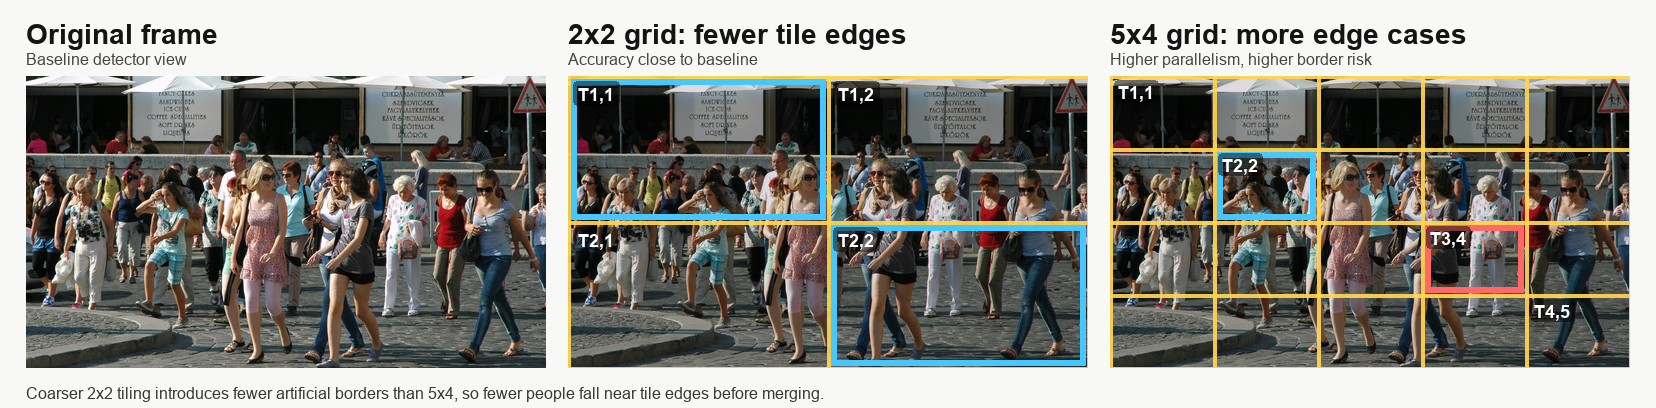
\includegraphics[width=0.98\textwidth]{figures/yolo_grid_split_visualization.png}
\caption{Hybrid temporal-spatial decomposition for YOLO video inference. The public-domain crowd frame is from Wikimedia Commons~\cite{keymeulen2011crowd}; the overlays show why coarse 2x2 tiling preserves accuracy better than finer 5x4 tiling while still creating independent frame-tile tasks.}
\label{fig:yolo-grid-split}
\end{figure}

\subsection{1D Mapping and Static Scheduling}
All frame-tile tasks are flattened into a one-dimensional list. For task index \(i\), chunk size \(k\), and \(P\) ranks, static block-cyclic scheduling assigns:
\begin{equation}
    owner(task_i) = \left\lfloor \frac{i}{k} \right\rfloor \bmod P.
\end{equation}
Static scheduling has low dispatch overhead because ranks can determine their own tasks locally. The measured repository results show that this advantage matters for the 600-frame 5x4 tiled YOLO workload.

\subsection{Communication and Merging}
After each rank finishes its assigned frame-tile tasks, it sends two types of data to rank 0: detected bounding boxes and timing metrics. The communication pattern is centralized. Worker ranks compute locally, then rank 0 gathers the local result payloads and performs the final merge.

For each detected person box, the worker stores:
\begin{equation}
    (frame\_id,\ tile\_id,\ x_1,\ y_1,\ x_2,\ y_2,\ score,\ class).
\end{equation}
The box coordinates are still relative to the local tile. Rank 0 first converts them back to original-frame coordinates:
\begin{equation}
    x^{global} = x^{local} + x_s,\qquad
    y^{global} = y^{local} + y_s,
\end{equation}
where \((x_s,y_s)\) is the top-left coordinate of the tile inside the original frame.

For each frame \(F_i\), rank 0 merges all detections from the \(R \times C\) tiles:
\begin{equation}
    B_i^{raw} = \bigcup_{j=1}^{RC} B_{i,j}.
\end{equation}
Since a person near a tile boundary may appear in more than one tile, duplicate boxes can occur. Rank 0 therefore applies tile-owner filtering followed by global non-maximum suppression:
\begin{equation}
    B_i^{final} = NMS(B_i^{raw}, \theta).
\end{equation}
The final people count for frame \(F_i\) is:
\begin{equation}
    count(F_i)=|B_i^{final}|.
\end{equation}
This centralized merge is necessary because each rank only sees its own assigned tiles, while duplicate removal requires all detections from the same frame.

\subsection{YOLO Algorithm Sketch}
\begin{algorithm}[H]
\caption{Static MPI YOLO people-counting pipeline}
\begin{algorithmic}[1]
\STATE Input video contains \(N\) frames; each frame is split into an \(R \times C\) grid.
\STATE Build task list \(\mathcal{T}\), where each task is \((frame\_id, tile\_id)\).
\STATE Flatten \(\mathcal{T}\) into a 1D list and assign task index \(q\) using
\[
    owner(q)=\left\lfloor \frac{q}{K} \right\rfloor \bmod P,
\]
where \(K\) is chunk size and \(P\) is the number of MPI ranks.
\FOR{each MPI rank \(r\) in parallel}
    \STATE Select all tasks whose owner is \(r\).
    \FOR{each selected task \((i,j)\)}
        \STATE Crop tile \(j\) from frame \(F_i\).
        \STATE Run YOLO inference on the tile.
        \STATE Keep only \code{person} detections.
        \STATE Store local boxes and timing metrics.
    \ENDFOR
\ENDFOR
\STATE Gather serialized detections and rank metrics to rank 0.
\IF{rank is 0}
    \FOR{each frame \(F_i\)}
        \STATE Convert tile-local boxes to global frame coordinates.
        \STATE Merge boxes from all tiles of frame \(F_i\).
        \STATE Apply tile-owner filtering and global NMS.
        \STATE Compute \(count(F_i)=|B_i^{final}|\).
    \ENDFOR
    \STATE Write per-frame counts and runtime metrics to CSV files.
\ENDIF
\end{algorithmic}
\end{algorithm}

\section{Parallel-Programming Focus}

\begin{table}[H]
\centering
\caption{Parallel-programming concepts in the YOLO MPI pipeline}
\label{tab:yolo-concepts}
\begin{tabularx}{\textwidth}{L{3.6cm} X}
\toprule
Concept & YOLO MPI implementation \\
\midrule

Parallelism level 
& Task-level parallelism: each task runs YOLO on one frame tile. \\

Decomposition 
& Hybrid temporal-spatial decomposition: video frames are divided into smaller image tiles. \\

Granularity
& Tile-level granularity: one task corresponds to one tile of one frame. \\

Mapping technique
& 1D task mapping: all frame-tile tasks are flattened into a list and assigned to MPI ranks using static block-cyclic distribution. \\

Communication strategy
& Each rank computes locally, then sends detections and timing results to rank 0 for merging. \\

Communication topology
& Master-worker topology: rank 0 gathers and post-processes results, while other ranks mainly perform inference. \\

Communication mode
& Blocking gather communication is used after local inference. \\

Load balancing
& Load balancing is considered through tile size, block-cyclic task assignment, and weighted process placement. \\

Correctness check
& The parallel output is correct if its frame-level people counts match the serial YOLO result after the same post-processing. \\

\bottomrule
\end{tabularx}
\end{table}
